%\documentclass{bsu-cs}  % default is thesis
%\documentclass[project]{bsu-cs}  % for project reports
%\documentclass[dissertation]{bsu-cs}  % for dissertation
\documentclass[project]{bsu-cs}  % for dissertation

%%%%%%%%%%%%%%%%%%%%%%%%%%%%%%%%%%%%%%%%%%%%%%%%%%%%%%%
% Only LaTeX commands (and whitespace) are allowed in the preamble.  A LaTeX
% command has the form
%
%   \<name>{<arg>}{<arg>}...
%
% where the number of arguments is set by the command definition. 
% Some commands allow an optional argument
%
%   \name[<opt>]{<arg>}{<arg>}...
%
% which may or may not be given.  There are also LaTeX environments
%
%   \begin{<name>}...\end{<name>}
%
% which can be nested, but must be balanced. 
%%%%%%%%%%%%%%%%%%%%%%%%%%%%%%%%%%%%%%%%%%%%%%%%%%%%%%%
% Packages
\usepackage[round]{natbib}
%\usepackage[dvips]{graphicx}
% Comment the above line and uncomment below to use pdflatex
\usepackage[pdftex]{graphicx}
% Then the figures should be in pdf, jpg or png format.

% Others to consider
\usepackage{listings}
\usepackage{color}
\definecolor{listinggray}{gray}{0.95}
\definecolor{mygreen}{rgb}{0,0.6,0}
\definecolor{mygray}{rgb}{0.5,0.5,0.5}
\definecolor{mymauve}{rgb}{0.58,0,0.82}
\definecolor{maroon}{rgb}{0.5,0.00,0.0}

\lstdefinestyle{javanonum}{
  backgroundcolor=\color{listinggray},   % choose the background color; you must add \usepackage{color} or \usepackage{xcolor}
  basicstyle=\footnotesize\ttfamily, % the size of the fonts that are used for the code
  breakatwhitespace=false,         % sets if automatic breaks should only happen at whitespace
  breaklines=true,                 % sets automatic line breaking
  captionpos=none,                 % sets the caption-position to bottom
  aboveskip=\smallskipamount,
  belowskip=\smallskipamount,      % default is \medskipamount
  commentstyle=\color{mygreen},    % comment style
  deletekeywords={...},            % if you want to delete keywords from the given language
  escapeinside={\%*}{*)},          % if you want to add LaTeX within your code
  extendedchars=true,              % lets you use non-ASCII characters; for 8-bits encodings only, does not work with UTF-8
  frame=none,                      % adds a frame around the code (none, single)
  keepspaces=true,                 % keeps spaces in text, useful for keeping indentation of code (possibly needs columns=flexible)
  keywordstyle=\color{maroon},       % keyword style
  language=Java,                   % the language of the code
  morekeywords={*,...},            % if you want to add more keywords to the set
  numbers=none,                    % where to put the line-numbers; possible values are (none, left, right)
  rulecolor=\color{black},         % if not set, the frame-color may be changed on line-breaks within not-black text (e.g. comments (green here))
  showspaces=false,                % show spaces everywhere adding particular underscores; it overrides 'showstringspaces'
  showstringspaces=false,          % underline spaces within strings only
  showtabs=false,                  % show tabs within strings adding particular underscores
  stringstyle=\color{mymauve},     % string literal style
  tabsize=4,                       % sets default tabsize to 4 spaces
% title=\lstname                   % show the filename of files included with \lstinputlisting; also try caption instead of title
}

\lstset{style=javanonum}

% If you want to use PostScript fonts (or the Nimbus knockoffs) try
\usepackage{mathptmx}
\usepackage[scaled=0.92]{helvet}

% The 'citesort' package puts mutliple citation numbers in order
% \usepackage{citesort}

\usepackage{hyperref}
\hypersetup{
	colorlinks=true,
	allcolors=blue,
}

%%%%%%%%%%%%%%%%%%%%%%%%%%%%%%%%%%%%%%%%%%%%%%%%%%%%%%%
% Local commands

%%%%%%%%%%%%%%%%%%%%%%%%%%%%%%%%%%%%%%%%%%%%%%%%%%%%%%%
% Front Matter Definitions
%%%%%%%%%%%%%%%%%%%%%%%%%%%%%%%%%%%%%%%%%%%%%%%%%%%%%%%

% These definitions are used by the commands below to construct the front 
% matter pages.  

% Document title
% The \titleBreak command produces a line break in the title on the
% title page (this may be necessary to keep longer titles from looking
% strange)
\title{Structured Reasoning in LLMs: A Synthesis of Methods and Future Directions}  

% Author's name (must be exactly what name the Registrar has)
% normally it is of the form "First Middle Last"
\author{Malia Rose Barker}  

% Day of oral defense
\defenseDate{<> November, 2025}

% % Month of graduation (do not abbreviate)
% \graduationMonth{December}

% % Year of graduation
% \graduationYear{2022} 

% Advisor (chair)
\advisor[Chair]{Edoardo Serra, Ph.D.}

% Committee members
\committeeA{Francesco Gullo, Ph.D.} 
\committeeB{Marion Scheepers, Ph.D.}
\committeeC[External Evaluator]{Grady Wright, Ph.D.}

% Full name of the degree
\degree{Doctor of Philosophy}

% Full name of major
\major{Computing (Data Science)}

% Major department
\department{Computer Science}

% College
\college{Engineering}

% Current department chair
\departmentChair{Jerry Fails}

% Document abstract
\abstract{ Text. }

% Acknowledgments
\acknowledgments{
This work is supported by the <> grant?
}

% (End of preamble)
%%%%%%%%%%%%%%%%%%%%%%%%%%%%%%%%%%%%%%%%%%%%%%%%%%%%%%%

\begin{document}

% The \frontmatter command prepares for front matter material
\frontmatter  %! Do not remove! 
% 
% The \buildFrontPages builds all the front matter pages
\buildFrontPages %! Do not remove! 
% 
% The (optional) list of abbreviations goes here
\begin{listAbbreviations}
  \item[LLM] Large Language Model
  \item[NLP] Natural Language Processing
  \item[CoT] Chain of Thought
  \item[LtM] Least to Most
  \item[ToT] Tree of Thoughts
  \item[GoT] Graph of Thoughts
\end{listAbbreviations}
% 
% The (optional) list of symbols goes here
% \begin{listSymbols}
%   \item[$\sqrt{2}$] square root of 2
%   \item[$\lambda$] lambda symbol, normally used in lambda calculus but
%     it sometimes gets used for wavelength as well
% \end{listSymbols}
% 
\mainmatter
% 
%%%%%%%%%%%%%%%%%%%%%%%%%%%%%%%%%%%%%%%%%%%%%%%%%%%%%
%
% Chapter: Introduction
%
%%%%%%%%%%%%%%%%%%%%%%%%%%%%%%%%%%%%%%%%%%%%%%%%%%%%%
% 
\chapter{Introduction} \label{ch:intro}
% 1 - 1.5 pages
Advancements in large language models (LLMs) have led to increased research blah blah idk. However, most language models lack the ability to reason and execute tasks based on their reasoning. Traditionally, improvements on models have been made through constant training and model parameter fine-tuning. However, collecting the large amounts of training data needed for these models is timely and costly depending on how the data is collected. Fine-tuning is also timely and computationally expensive, and fine-tuning can also influence the final model towards a bias, leading to models that do not generalize well to newly introduced data. 
% TODO: maybe add some citations here that back up the claims: "do not reason well", "data collection is expensive", and "fine-tuning does not generalize well"

In recent years, researchers have developed a new method of forcing models to reason with no additional training or fine-tuning called prompting or prompt engineering. Prompting involves creating a prompt or query to pass to the LLM, affecting the LLM's output directly. For example, to force an LLM to reason through a problem instead of just outputting an answer, one could simply tack on "Let's think through this step-by-step," to the end of the initial prompt \citep{kojima2023largelanguagemodelszeroshot}. Prompting consists of zero-shot, which is demonstrated by the former example, and few-shot, which includes one or more examples of structured reasoning that the user would like the LLM to execute. A comparison of zero-shot vs. few-shot prompting is provided in Figure \ref{fig:}.

In-context learning/few-shot learning takes place at inference time, meaning no parameters of the model are changed.
% TODO: Insert figure of zero vs few-shot prompting and finish reference above.
% 
% LLMs are big, however they are bad at reasoning. There are a few ways to imrpove this, including more training data, fine-tuning models, prompt engineering. Training data and fine-tuning models is computationally costly and can lead to overfitting problems or non-generalizable models, which isn't ideal for future applications where data may be not as similar as original trainign set or what model was fine-tuned on. Prompting however take a different approach in that it doesn't alter the model at all, but instead the input/output of the model. This allows the forcing of reasoning abilities for off-the-shelf models. Let's go into the different frames of prompting.
\begin{enumerate}
    \item Problem framing: LLMs excel at language fluency but fail at robust reasoning.
    
    \item Motivation: Why reasoning matters (math, science, planning, real-world decision-making).
    
    \item Motivate the central question: “How do large language models perform complex reasoning, and what mechanisms improve reliability and compositionality?”

    \item Explain that recent advances extend CoT prompting toward structure, reflection, and verifiability.

    \item Across prompting methods, the core strategy is making reasoning explicit (externalizing hidden steps into observable traces).

    \item Preview your organizational lens: token-based reasoning → structured decomposition → executable and agentic reasoning.

    \item Emphasize that this review traces that evolution.
\end{enumerate}
% 
\chapter{Relevant Works}\label{ch:works}
%%%%%%%%%%%%%%%%%%%%%%%%%%%%%%%%%%%%%%%%%%%%%%%%%%%%%
%
% Section: Token-Based Reasoning: CoT & Extensions
%
%%%%%%%%%%%%%%%%%%%%%%%%%%%%%%%%%%%%%%%%%%%%%%%%%%%%%
\section{Token-Based Reasoning: The Chain-of-Thought Paradigm}\label{sec:CoT}
% 
\begin{figure}
    \centering
    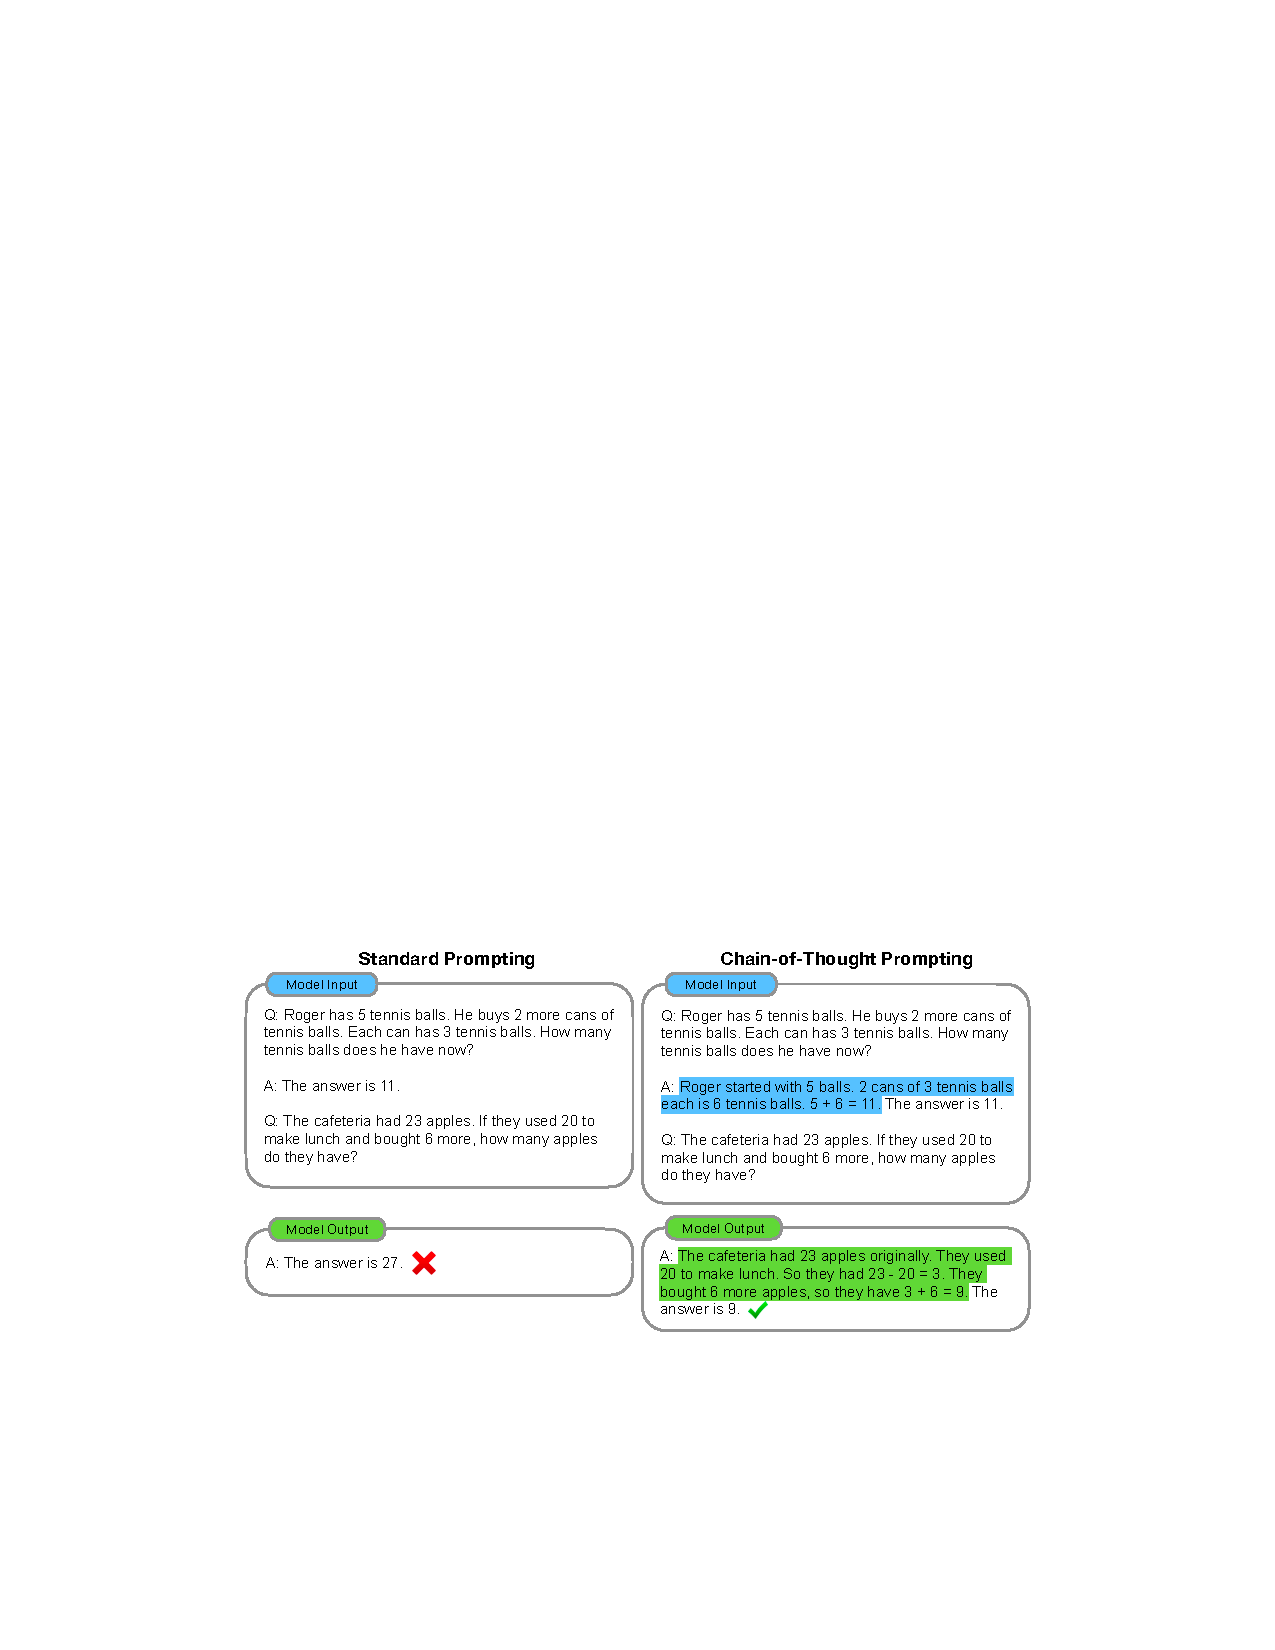
\includegraphics[width=0.8\linewidth]{figures/cot1.pdf}
    \caption{From \citet{DBLP:journals/corr/abs-2201-11903}: comparison of a standard few-shot prompt versus a chain-of-thought (CoT) few-shot prompt.}
    \label{fig:cot1}
\end{figure}
% 
Language models generate sequences of tokens, where each token may correspond to a fragment of reasoning or a “thought.” Early prompting strategies, such as those introduced by \citet{DBLP:journals/corr/abs-2005-14165}, demonstrated that few-shot examples alone could substantially improve task performance. Building on this insight, \citet{DBLP:journals/corr/abs-2201-11903} proposed \textit{Chain-of-Thought} (CoT) prompting, which explicitly encourages models to reason step by step. As shown in Figure~\ref{fig:cot1}, including a single example of intermediate reasoning in the prompt yields large performance gains across arithmetic, symbolic, and commonsense reasoning tasks by eliciting structured intermediate steps in the model’s output. Across datasets such as GSM8K and MultiArith, CoT prompting improved accuracy by over 40\% compared to standard few-shot baselines when applied to large models such as GPT-3 (175B) and PaLM (540B).

Following this discovery, \citet{wang2023selfconsistencyimproveschainthought} introduced \textit{Self-Consistency}, a simple but powerful extension in which multiple reasoning paths are sampled, and the final answer is chosen by majority vote among consistent outputs. The key idea is to increase diversity among reasoning chains by sampling from the model at a higher \textit{temperature}—a parameter that controls randomness during generation. Higher temperatures cause the model to explore a wider range of plausible reasoning trajectories instead of repeating similar outputs each time. This diversity allows the method to identify reasoning paths that converge on the same final answer while filtering out inconsistent or implausible ones. The intuition parallels human reasoning: the path that most frequently leads to the same conclusion is likely to be correct, whereas erroneous reasoning chains are unlikely to recur. This self-ensemble approach further improves robustness and accuracy relative to single-pass CoT prompting, yielding an average accuracy gain of roughly 18\% on the GSM8K dataset compared to CoT alone.

CoT marks a major shift in how reasoning is elicited from LLMs—transforming them from opaque black boxes into systems that externalize intermediate steps in a human-verifiable form. However, these reasoning traces remain purely linguistic: their correctness can be judged by humans but not easily verified by machines. Few-shot exemplars also require manual curation or generation, which limits scalability and introduces bias toward the chosen examples. Zero-shot CoT methods, such as the “Let’s think step by step” approach proposed by \citet{kojima2023largelanguagemodelszeroshot}, partially mitigate this issue by removing the need for curated demonstrations. Yet even without exemplars, the resulting reasoning remains expressed entirely in natural language, making it difficult to verify or standardize automatically.
% TODO: Include a citation on that paper that shows that these prompting strategies are sensitive to exemplar choices?

Moreover, both CoT and Self-Consistency primarily demonstrate success on structured mathematical or symbolic benchmarks, where intermediate reasoning steps map cleanly onto ground-truth solutions. These tasks are well-suited to CoT because they inherently require multi-step reasoning and offer clear verification targets. By contrast, open-ended natural language reasoning—such as question answering or dialogue—poses additional challenges, as intermediate steps are less formally constrained and harder to evaluate automatically. Compounding this issue, reasoning chains expressed in natural language remain vulnerable to hallucinations, inconsistencies, and arithmetic errors, with no built-in mechanism for self-correction. As a result, while CoT and Self-Consistency establish a strong baseline for explicit reasoning and interpretability, their limitations highlight the need for more structured and verifiable reasoning frameworks—motivating the structured decomposition and search methods discussed next.
% 
%%%%%%%%%%%%%%%%%%%%%%%%%%%%%%%%%%%%%%%%%%%%%%%%%%%%%
%
% Section: Structured Decomp & Search
%
%%%%%%%%%%%%%%%%%%%%%%%%%%%%%%%%%%%%%%%%%%%%%%%%%%%%%
% 
\section{Structured Decomposition and Search in Thought Space}\label{sec:decomp}
% 
The evolution from Chain-of-Thought to more structured reasoning reflects a shift from eliciting reasoning to organizing it. While CoT and Self-Consistency make reasoning explicit, they do so only at the level of language: steps are sequential but unstructured, and no mechanisms exist to plan or evaluate intermediate results. To address these challenges, recent approaches such as Least-to-Most (LtM) \citep{zhou2023leasttomostpromptingenablescomplex}, Tree-of-Thought (ToT) \citep{yao2023treethoughtsdeliberateproblem}, and Graph-of-Thought (GoT) \citep{Besta_2024} introduce explicit structure into the reasoning process by decomposing tasks into smaller subproblems or systematically searching over alternative reasoning paths. These methods extend the interpretability of CoT while aiming for more consistent, compositional, and verifiable reasoning.

\begin{figure}
    \centering
    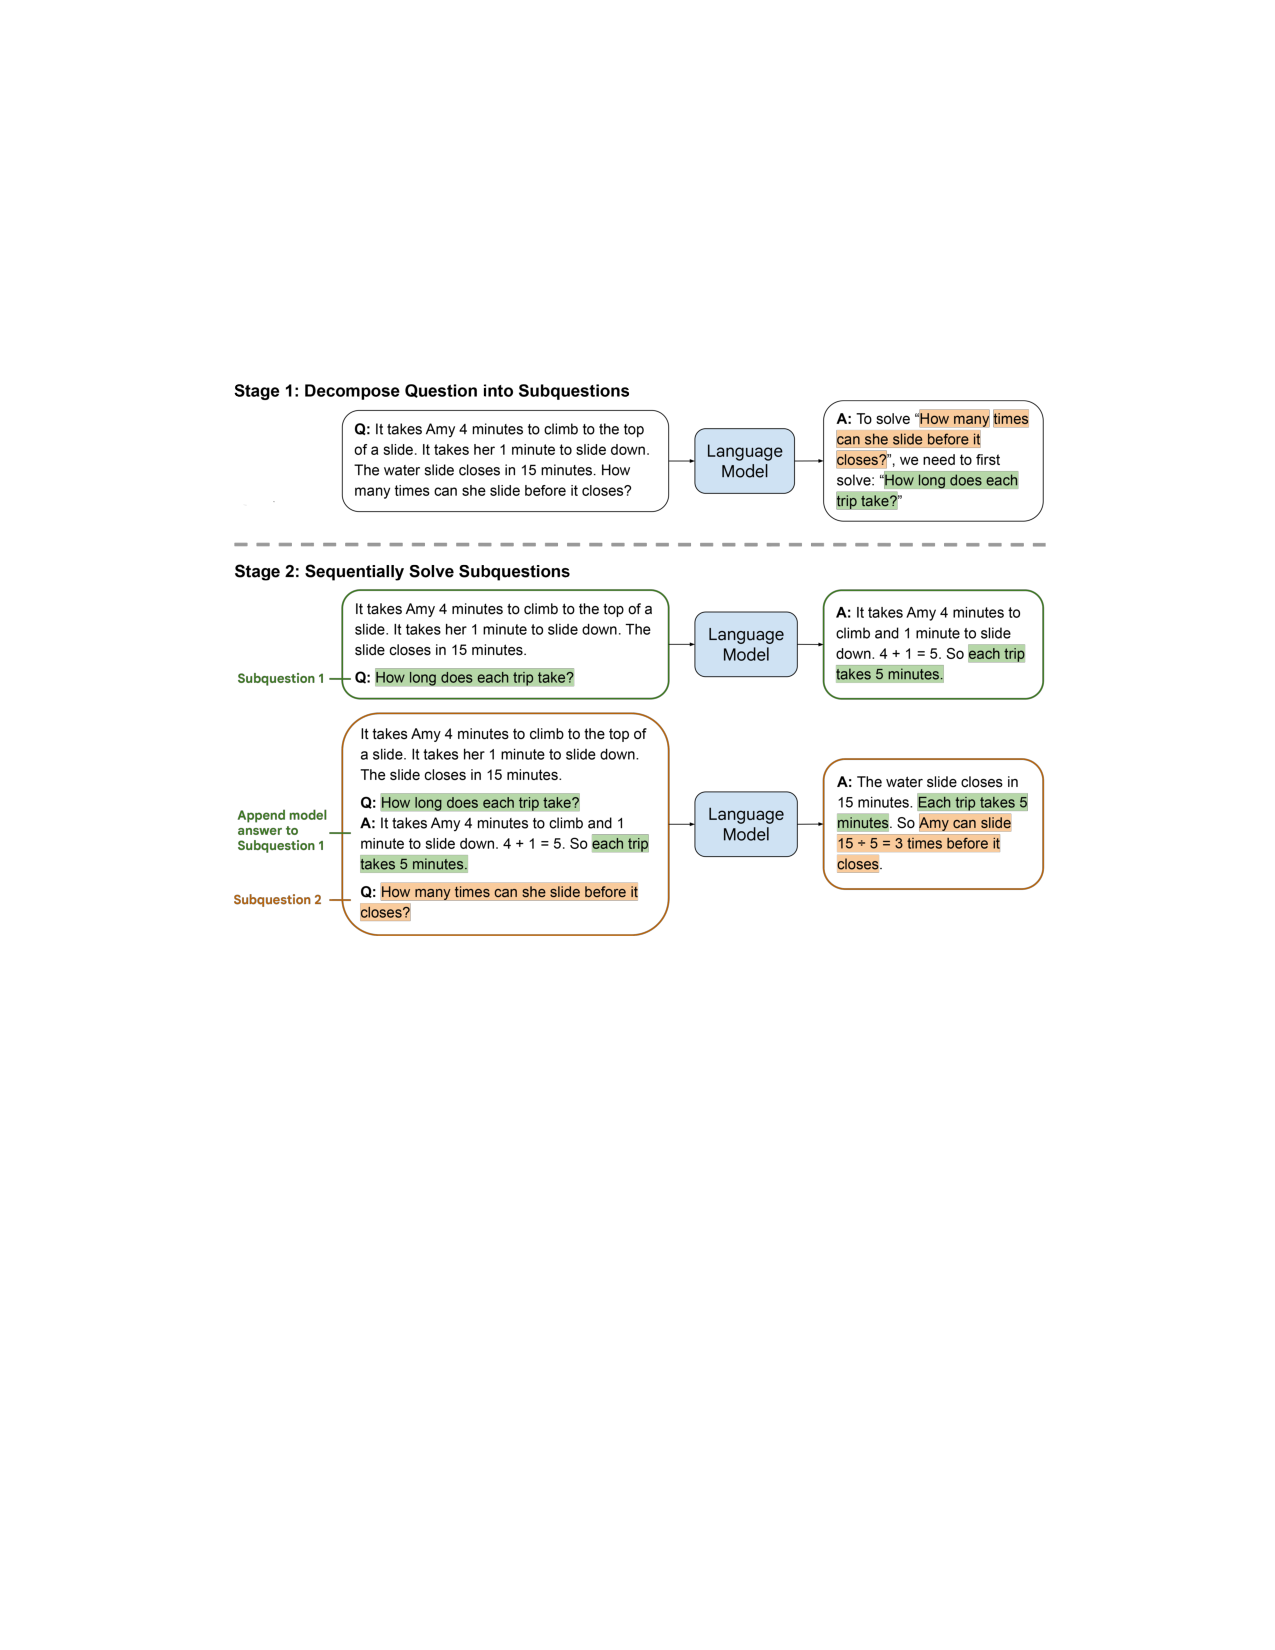
\includegraphics[width=0.8\linewidth]{figures/ltm1.pdf}
    \caption{From \citet{zhou2023leasttomostpromptingenablescomplex}, an example of the sub-problem decomposition approach taken by Least-to-Most prompting for a math word problem.}
    \label{fig:ltm1}
\end{figure}

LtM prompting decomposes the original question into a list of subproblems to solve linearly, whereby solving a given subproblem is facilitated by answers to previously solved subproblems. In tackling the questions bu decomposition, LtM allows the LLM to generalize better, enabling the LLM to overcome easy-to-hard generalization in which the test problems are harder to solve than the example problems. While overall improvements are minimal when compared to CoT prompting, harder questions such as GSM8K questions that decompose into 5 or more steps show a <>\% improvement, showcasing the generalizability that LtM provides over CoT. However, this does not mean that it improves generalizability overall, as the decomposition prompts do not generalize well across domains and can even have difficulty generalizing within the same domain, possibly explaining why there is not such a large increase on the GSM8K dataset as there was on other datasets. Furthermore, generated thoughts still exist in a text-token space, making it hard to verify and search over the reasoning space.

\begin{figure}
    \centering
    \includegraphics[width=0.5\linewidth]{}
    \caption{Caption}
    \label{fig:placeholder}
\end{figure}

Tree of thoughts and graph of thoughts both aim to tackle complex searches in the thought token space, allowing exploration over different reasoning chains with lookahead and backtracking. In human cognitition, "dual process" models exhibit two levels of thinking: system 1, which includes fast, automatic, and unconscious thinking, can best describe how most LLMs reach their conclusions while system 2, which includes slow, deliberate, and conscious thinking, contributes to planning and tracking. The goal in adding more structure through ToT and GoT is to enforce a system 2 level of thinking in the LLM, forcing it to make deliberate decisions in its reasoning process by considering multiple different reasoning paths and self-evaluating choices to decide the next course of action. This also contributes to increased generality, allowing for improvements on NLP tasks such as creative writing and solving crosswords, with the latter benchmark exhibiting a 60\% word-level success rate while CoT exhibits a mere 16\% word-level success rate.

GoT further improves on this while also reducing costs by greater than 31\% \citep{Besta_2024}. Furthermore, GoT better utilizes self-reflection, allowing the LLM to loop over a thought if refinement is deemed necessary.

These methods show increased structure in reasoning and generalizability by exploring the thought space systematically, constraining reasoning while still allowing outputs to be text-based and therefore easily interpretable. However, they still lack the verifiable structure needed to ground the LLM's reasoning and reduce hallucinations. While GoT reduces computational costs compared to previous methods, it is still computationally expensive to explore the thought space when compared to simple input-output LLM execution. Furthermore, these methods lack standardization, making it hard to repurpose thought traces which may have been costly to create and recreate when they are needed again. These methods operate in thought space—searching over natural-language reasoning traces—but do not explore procedure space, where reasoning is represented in structured, executable forms.

\begin{enumerate}
    \item Least-to-Most \citep{zhou2023leasttomostpromptingenablescomplex} — linear decomposition, smaller subproblems.

    \item Tree-of-Thought \citep{yao2023treethoughtsdeliberateproblem} — branching reasoning with search algorithms, explicit search over reasoning paths.

    \item Graph-of-Thought \citep{Besta_2024} — generalized, flexible graph structures, compositional reasoning, and dynamic dependencies.

    \item Comparative analysis: how these methods explore thought space systematically. All try to constrain reasoning, but outputs remain text-based.

    \item Limitations: structure without semantics; steps not executable or verifiable, computational cost, lack of standardization, hard to repurpose traces.

    % \item Later linkage: you’ll position your work as a shift from “thought-structure” to “procedure-structure.”
\end{enumerate}
% 
%%%%%%%%%%%%%%%%%%%%%%%%%%%%%%%%%%%%%%%%%%%%%%%%%%%%%
%
% Section: Programmatic and Executable Reasoning
%
%%%%%%%%%%%%%%%%%%%%%%%%%%%%%%%%%%%%%%%%%%%%%%%%%%%%%
% 
\section{Programmatic and Executable Reasoning}\label{sec:programmatic}
% 1.5 - 2 pages
\begin{enumerate}
    \item PAL \citep{gao2023palprogramaidedlanguagemodels} (LLM generates code, external executor solves) and Program of Thoughts \citep{chen2023programthoughtspromptingdisentangling} (hybrids of code + natural language steps): LMs generating code to perform reasoning.

    \item Discuss how this introduces verifiability through execution — but at the cost of brittleness and modality-switching.

    \item Contrast symbolic execution with natural-language decomposition.

    \item Highlight the beginning of reasoning as explicit programs/procedures.

    \item Strengths: precise, verifiable execution for math/logical tasks.

    \item Limitations: narrow domain (requires formalizable problems), not directly generalizable to abstract reasoning.

    % \item Later linkage: precursor to your “search in procedure space” idea.
\end{enumerate}

EA sentence: A related direction involves search and optimization over generated programs or solutions. Systems such as LLaMEA \citep{zhou2024llamea} and FunSearch \citep{rombach2024funsearch} pair LLMs with evolutionary or search-based evaluators that optimize generated code for correctness or performance. These frameworks demonstrate how programmatic reasoning can be evolved and verified through iterative feedback, bridging the gap between textual reasoning and executable evaluation.
% 
%%%%%%%%%%%%%%%%%%%%%%%%%%%%%%%%%%%%%%%%%%%%%%%%%%%%%
%
% Section: Agentic and Reflective Reasoning
%
%%%%%%%%%%%%%%%%%%%%%%%%%%%%%%%%%%%%%%%%%%%%%%%%%%%%%
% 
\section{Agentic and Reflective Reasoning}\label{sec:reasoning}
% 1.5 - 2 pages
\begin{enumerate}
    \item ReAct \citep{yao2023reactsynergizingreasoningacting} — reasoning + acting loops.

    \item Reflexion \citep{shinn2023reflexionlanguageagentsverbal} — self-evaluation and learning from feedback across episodes.

    \item Optionally include Self-Refine \citep{madaan2023selfrefineiterativerefinementselffeedback} or AutoGen \citep{wu2023autogenenablingnextgenllm} for multi-agent/feedback coordination.

    \item \citet{lightman2023letsverifystepstep} introduced a verbal reinforcement learning framework in which a model iteratively critiques its own intermediate steps (“Let’s Verify Step by Step”). This method achieves stronger reasoning consistency by training models to generate verification statements. However, the validation remains linguistic rather than executable—verification occurs in natural language rather than through formal or symbolic checks. In contrast, emerging approaches seek machine-checkable validation, where reasoning steps can be executed or structurally verified without additional model training.
    % In future Related Work: reuse the same paragraph to delineate verbal RL-based validation (training-dependent) vs. procedure-based validation (training-free, structural).
    \item Emphasize interaction and feedback loops: models as agents that reason, act, and self-correct iteratively.

    \item Limitations: reasoning traces exist but are inconsistent, no universal format (these systems still operate mostly over textual reasoning traces, not structured procedures).

    % \item Later linkage: your “typed reflection + validator feedback” mechanism builds directly on this lineage.
\end{enumerate}
% 
%%%%%%%%%%%%%%%%%%%%%%%%%%%%%%%%%%%%%%%%%%%%%%%%%%%%%
%
% Section: Search and Optimization in Reasoning Space
%
%%%%%%%%%%%%%%%%%%%%%%%%%%%%%%%%%%%%%%%%%%%%%%%%%%%%%
% 
\section{Search and Optimization in Reasoning Space}\label{sec:opt}
\begin{enumerate}
    \item Define the difference between searching over text/thoughts (ToT, GoT) vs. searching over generated artifacts (programs, procedures).

    \item Summarize LLaMEA, FunSearch, and EvoPrompt as early explorations of this.

    \item Mention how these methods “close the loop” between reasoning generation and validation.

    \item End with: “However, these approaches remain primarily token- or code-based, rather than operating over structured, verifiable procedures that generalize reasoning as modular, composable actions.”
\end{enumerate}
% 
%%%%%%%%%%%%%%%%%%%%%%%%%%%%%%%%%%%%%%%%%%%%%%%%%%%%%
%
% Section: Toward Structured, Verifiable, and Agentic Reasoning
%
%%%%%%%%%%%%%%%%%%%%%%%%%%%%%%%%%%%%%%%%%%%%%%%%%%%%%
% 
\section{Toward Structured, Verifiable, and Agentic Reasoning}\label{sec:struct}
% 2 - 2.5 pages
\subsection{Trends in Structured Reasoning}
\begin{enumerate}
    \item Synthesize trends: From token-level → structural decomposition → executable and agentic reasoning. Increasing emphasis on validation, control, and interpretability.

    \item Identify the open gap: Existing frameworks lack machine-checkable structure and validator-based pruning. “Search in token/thought space” does not equal “search in procedure space.”

    \item Introduce the conceptual frontier: Procedural reasoning, verifiability, and integration of agentic feedback loops.

    % \item Later linkage: this becomes the last paragraph of your “Related Work” section that motivates your contribution.
\end{enumerate}
% 
\subsection{The Emerging Frontier}
\begin{enumerate}
    \item Process Reward Models \citep{lightman2023letsverifystepstep}: supervise intermediate steps, not just final answers.

    \item Instruction-tuned datasets (MathInstruct, OpenMathInstruct, InfinityMath): large-scale corpora mixing CoT and code reasoning.

    \item Synthesis: promising move toward reasoning as trainable signal.

    \item Limitations: reasoning traces are still free-form, noisy, and not standardized.
\end{enumerate}
End sentence: “An open question remains: how can reasoning be represented as procedures that are both interpretable to humans and verifiable by machines, and how might such structures be optimized automatically without retraining models?”
% 
%%%%%%%%%%%%%%%%%%%%%%%%%%%%%%%%%%%%%%%%%%%%%%%%%%%%%
%
% Chapter: Conclusion
%
%%%%%%%%%%%%%%%%%%%%%%%%%%%%%%%%%%%%%%%%%%%%%%%%%%%%%
% 
\chapter{Conclusion}\label{ch:conclusion}
% 1 page
\begin{enumerate}
    \item Shared insight/summary: Forcing explicit reasoning improves accuracy. Explicit reasoning is essential but unresolved in its best form.

    \item Differences across methods:
    \begin{itemize}
        \item CoT/CoT-SC → introduces interpretability, simple but messy.

        \item Structured search/prompting (LtM/ToT/GoT) → adds compositional reasoning, more systematic but heavy.

        \item Programmatic → precise but narrow.

        \item ReAct/Reflexion → agentic feedback brings adaptivity, dynamic but agent-oriented and still token-based search.
        % IDK if I'll include this because I don't really review these unless I do wanna include the lightman paper
        % \item PRMs/Datasets → scalable but lack consistent representation.
    \end{itemize}

    \item Critical synthesis: No consensus yet on the “best” representation of reasoning; each approach balances structure, verifiability, and generality differently.

    \item Takeaway: Field is converging on structured, verifiable reasoning traces, but challenges remain in standardization, efficiency, and trainability. Verifiable structure and execution-based validation remain underexplored.

    \item Future directions (general, not your work):

        \subitem More structured representations of reasoning.

        \subitem Scalable process-level supervision.

        \subitem Benchmarks that test reasoning robustness, not just accuracy.
\end{enumerate}
End sentence: “Future systems may integrate structured procedural representations with optimization and feedback mechanisms — enabling models not just to reason in language, but to evolve verifiable reasoning procedures autonomously.”
% 
\backmatter
%%%%%%%%%%%%%%%%%%%%%%%%%%%%%%%%%%%%%%%%%%%%%%%%%%%%%%
%
% Bibilography
%
%%%%%%%%%%%%%%%%%%%%%%%%%%%%%%%%%%%%%%%%%%%%%%%%%%%%%%
\bibliographystyle{plainnat}
\bibliography{bibliography.bib}
%%%%%%%%%%%%%%%%%%%%%%%%%%%%%%%%%%%%%%%%%%%%%%%%%%%%%%%
%
% Appendix
%
%%%%%%%%%%%%%%%%%%%%%%%%%%%%%%%%%%%%%%%%%%%%%%%%%%%%%%%
\appendix
% After \appendix has executed, the \chapter command creates an appendix.
% Appendices are numbered by "A", "B", etc.
% \chapter{Timing Measurements}\label{app:Timing}
% Here is Appendix A. See Appendix~\ref{app:Setup} for the experimental setup.
\finish  %! Do not remove!

\end{document}

%  LABELS
%   ch:<name>  for chapters
%   sec:<name> for sections
%   tbl:<name> for tables
%   fig:<name> for figures

% CITATIONS
% \cite{<tag>} is bibilography citation; <tag> must match a bibliography
% item label.  It can take multiple, comma-separated, arguments.

% The '~' is a "tie", which is an unbreakable space.  That is, it is
% the same a a space but TeX won't break the line there.  Ties are used
% between text and a reference or citation, to avoid something like Figure
% 1, which looks weird.

% TEXT FORMATTING
% \texttt{} changes to "typewriter" (monospaced) font, which is typically
% used for literal code or filenames.
% \emph{} "emphasizes" the text, which normally means placing it in
% italics if the running text is in Roman font, or vice-versa.

% FOOTNOTES
% So here is some extra stuff:%
% \footnote{Too many footnotes, however, can be distracting.}
% A '%' comment character at the end of a line, like above, has the
% effect of "escaping" the newline, thereby avoiding adding a space.
% In this case, it prevents there being space between the end of the
% text and the footnote superscript
%! The \label command applies to the most recent heading in the main text,
%! or the current figure or table.  
%! The \pageref{<tag>} command references the page number of a label.
% Check the References on page~\pageref{references} for an example of how to format the references.

% \textbf{} sets text in bold face.  It is useful in headings, but
% is rarely used in running text.  It is used here to denote literal
% LaTeX commands, and to illustrate its use.  Normally it is preferable
% to use \emph{} to emphasize text.
% When showing a program fragment, use the \textbf{verbatim} environment. However, when you wan
% to show an algorithm, use either the \textbf{tabbing} or \textbf{algorithm} environment.

% Thesis and dissertation text is normally ``double'' spaced.  It is customary to single-space
% literal code.  Figure~\ref{fig:code} shows a sample Java program.

% You can control, to some degree, where floating elements go by setting
% the optional argument of \begin{figure}.  The options are
%
%   h - place the figure at this point, if possible (avoid this)
%   t - place the figure at the top of a page
%   b - place the figure at the bottom of a page
%   p - place the figure on a special page containing only figures and tables
%
% The options can be combined, and a '*' can be appended to make LaTeX
% try harder to match the request.  For example, \begin{figure}[tp*]
% allows the figure to be placed at the top of the page or on a special
% page ([tp*] is in fact the default set in "bsu-cs.cls").  Avoid using
% [h] by itself--it is inflexible and can cause formatting problems.  At
% the same time, it can be very useful in forcing figure placement.
% Finessing figure placement is a typesetting task that you just have to get 
% used to, no matter what system you are using.  

% \begin{vcode}  
% % an alternative to 'singlespace', that also shrinks the
% % typewriter font so that it blends better with the text
% \begin{lstlisting}
% /**
% Compute x^n using recursive doubling technique. O(lg n) multiplications.
% @param x  The base value, unlimited precision.
% @param n  The exponent, an integer.
% @return   The computed power as a BigInteger
% */
% public static BigInteger power(BigInteger x, int n)
% {
%     BigInteger temp = x;
%     BigInteger result = BigInteger.ONE;
% 	while (n != 0) {
%         if ((n & 1) == 1) 
%             result = result.multiply(temp);
% 		if ((n = n >>>1) != 0)
%            	temp = temp.multiply(temp);
%     }
%     return result;
% }
% \end{lstlisting}
% \end{vcode}

%\caption{} gives the figure or table a caption, which is normally
% placed below the figure (but above a table).  The caption is also
% used as the title of the figure in the list of figures.  An optional
% argument gives the figure a "short title" for use in the list of
% figures, which is useful if the caption is long, or includes some
% extra information.
% \begin{figure}[t]
% \caption[Repeated Squaring Power Method]{Repeated Squaring Power Method. This figure
% also serves as an example of the inclusion of literal code.}
% \label{fig:code} 
% \end{figure}
%
% WARNING: the labels can get screwed up if the label in a figure is given
%          before the caption (another one of LaTeX's quirks)

% Tables are like figures, except that they are numbered separately
% and the caption is placed at the top.  Also there is a separate
% list of tables in the front matter.

% Here is a simple table.

% \begin{table}[h] % 'h' in this case prevents the table from being placed
                 % too close to the figure
% By custom, the caption of a table is placed at the top of the table.
% \caption{The Approximate Time of Parallelizing Each Code}
% (The label must follow the caption)
% \label{table4}
% \centering % tables need be horizontally centered
% The 'tabular' environment can be used to format tables.  Unfortunately
% it is one of the more cumbersome LaTeX constructs.
% \begin{tabular}{|c|c|c|c|}\hline \hline
% Parallel library/language  &WRS Code  &OCS Code  &ICSAMD Code\\ \hline
% MPI                        &20 hours  &2 weeks   &1 month\\ \hline
% HPF                        &3 hours   &1 1/2 weeks  &1 month\\ \hline
% \end{tabular}
% \end{table}

% \begin{figure}[h]
% % Code in figures is normally not centered, but graphical figures are
% % (the \centering command works as well as the 'center' environment, 
% % because its scope is limited to the figure).
% \begin{center}
% \includegraphics*[width=4.0in,keepaspectratio]{figure}
% \end{center}
% \caption{How to Correct Errors in a Fuzzy Image}
% \label{fig:fuzzyImage}
% \end{figure}

% \begin{table}[ht]
% \caption{Complexity of Selection and Search in Sorted Matrices}
% \label{tbl:CSSSM}
% \centerline{
% \begin{tabular}{|l|cccc|}
% \hline
% & Sorted $X+Y$ & \multicolumn{2}{c}{Matrix with sorted rows} & Matrix with sorted \\ 
% &  & \multicolumn{2}{c}{and sorted columns} & columns \\ \cline{2-5}
% & $|X|=|Y|=n$ &  $n \times m$, $m \leq n$ & $n \times n$ & $n \times m$ \\ 
% \hline
% $k = \Theta(mn)$ or $\Theta(n^2)$ & $\Theta(n)$ & $\Theta(m
% \log (2n/m))$ & $\Theta(n)$ & $\Theta(m \log n)$ \\
% \hline
% \end{tabular}
% }
% \end{table}